\section{More Details on Secondary Analyses}
\label{app:secondary-analyses}

\subsection{Aggregation Strategies for Expert Rankings}
\label{app:aggregation_strategies}

To account for residual variability across expert judgments, we construct multiple partial rankings using different aggregation strategies, as summarized in Table~\ref{tab:expert_aggregation}. These strategies capture varying levels of consensus, ranging from strict agreement to more relaxed formulations that allow ties or limited violations.

The number of resulting rankings differs substantially across strategies, reflecting the degree of flexibility each approach permits. Together, these aggregated rankings provide a principled way to model expert uncertainty and are used as alternative ground truths in our subsequent analysis.

\begin{table}[t]
\centering
\scriptsize
\begin{tabular}{lcl}
\toprule
\textbf{Strategy} & \textbf{\# Rankings} & \textbf{Representative Rankings} \\
\midrule
Strict & 4 &
$\{[1,4,7,6], [1,5,7,6], [2,4,7,6], [2,5,7,6]\}$ \\

Unanimous up to ties & 6 &
$\{[1,2,4,7,6], [1,2,4,7,8], [1,2,5,3,6], \dots\}$ \\

1 violation & 14 &
$\{[1,2,4,5,7,6], [1,2,4,5,7,8], [1,2,4,7,6,8], \dots\}$ \\

Majority & 1 &
$\{[1,2,5,4,3,7,8,6]\}$ \\
\bottomrule
\end{tabular}
\caption{Partial rankings derived from different expert aggregation strategies. The table reports the number of valid rankings per strategy and representative examples; full sets are used in the analysis.}
\label{tab:expert_aggregation}
\end{table}

\subsubsection{Expert Ranking Aggregation and Correlation Analysis}

\paragraph{Expert Rankings}
Let
\[
S = \{1, 2, \dots, 8\}
\]
denote the set of code snippets used in the study.

Each expert provides a ranking over the snippets, allowing for ties.  
We model an expert’s judgment as a binary preference relation
\[
\prec_e \;\subseteq\; S \times S,
\]
where \( a \prec_e b \) means that expert \( e \) considers snippet \( a \) easier to understand than snippet \( b \).
If an expert judges two snippets to be equally difficult, neither ordering is included.

Given a candidate aggregated ranking
\[
R = (r_1, r_2, \dots, r_k),
\]
we say that \( R \) induces the pairwise relation
\[
r_i \prec_R r_j \quad \text{iff} \quad i < j.
\]

Our goal is to construct aggregated expert rankings under different consistency assumptions and then correlate them with rankings derived from student data. In our setting, the rankings produced by Strategy~4 (pure majority aggregation) and Strategy~5 (mean-rank aggregation) are identical. Therefore, we report their results jointly under the label \emph{majority/mean}.

\subsubsection{Aggregation Strategies for Expert Rankings}

We consider five aggregation strategies, each imposing different constraints on how expert preferences must align with the aggregated ranking.

\paragraph{Strategy 1: Strict Unanimous Agreement}
A ranking \( R \) satisfies \emph{strict unanimous agreement} if for every induced pair \( (a,b) \in \prec_R \),
\[
\forall e \in E:\quad a \prec_e b.
\]

That is, all experts must strictly agree on the ordering of every pair in \( R \).
Ties are not permitted for any included comparison.
This is the strongest notion of consensus and typically yields short rankings.

\paragraph{Strategy 2: Unanimous Agreement up to Ties}
A ranking \( R \) satisfies \emph{unanimous agreement up to ties} if for every induced pair \( (a,b) \in \prec_R \),
\[
\forall e \in E:\quad \neg(b \prec_e a).
\]

Experts may either agree that \( a \) is easier than \( b \) or consider them tied, but no expert may express the opposite preference.
This strategy relaxes strategy~1 by allowing ties while still excluding contradictions.

\paragraph{Strategy 3: Unanimous up to Ties with One Global Violation}
A ranking \( R \) satisfies strategy~3 if it violates the strategy~2 condition for \emph{at most one unordered pair} \( \{a,b\} \subseteq R \).
Formally, there exists at most one pair such that
\[
\exists e \in E:\quad b \prec_e a,
\]
while all other pairs satisfy the strategy~2 constraint.

This strategy captures rankings that are nearly unanimous while permitting a single global inconsistency, enabling longer rankings.

\paragraph{Strategy 4: Pure Majority Aggregation}
For any pair \( (a,b) \), define the majority preference relation:
\[
a \prec_{\text{maj}} b
\quad \text{iff} \quad
|\{e \mid a \prec_e b\}| > |\{e \mid b \prec_e a\}|.
\]

A ranking \( R \) is valid under pure majority aggregation if all its induced pairs are consistent with \( \prec_{\text{maj}} \).
This approach allows disagreement among experts and corresponds to classical majority voting.
Because majority relations may contain cycles, not all snippets can necessarily be included.

\paragraph{Strategy 5: Mean-Rank (Borda-Style) Aggregation}
Let \( \text{rank}_e(a) \) be the numeric rank assigned to snippet \( a \) by expert \( e \), with tied snippets receiving equal ranks.
The mean rank of snippet \( a \) is
\[
\overline{\text{rank}}(a) = \frac{1}{|E|} \sum_{e \in E} \text{rank}_e(a).
\]

The aggregated ranking is obtained by sorting snippets in increasing order of \( \overline{\text{rank}}(a) \).
This method produces a single total order over all snippets and serves as a baseline aggregation strategy.

\subsubsection{Selection of Expert Rankings for Analysis}

For each aggregation strategy, we enumerated all valid rankings and selected those with \emph{maximum length} (i.e., containing the largest number of snippets).
These longest rankings were used for correlation analysis, as they maximize comparability with student-derived rankings while respecting the defining constraints of each strategy.

% =====================================================
\subsubsection{Results}
% =====================================================

\begin{figure}[t]
    \centering
    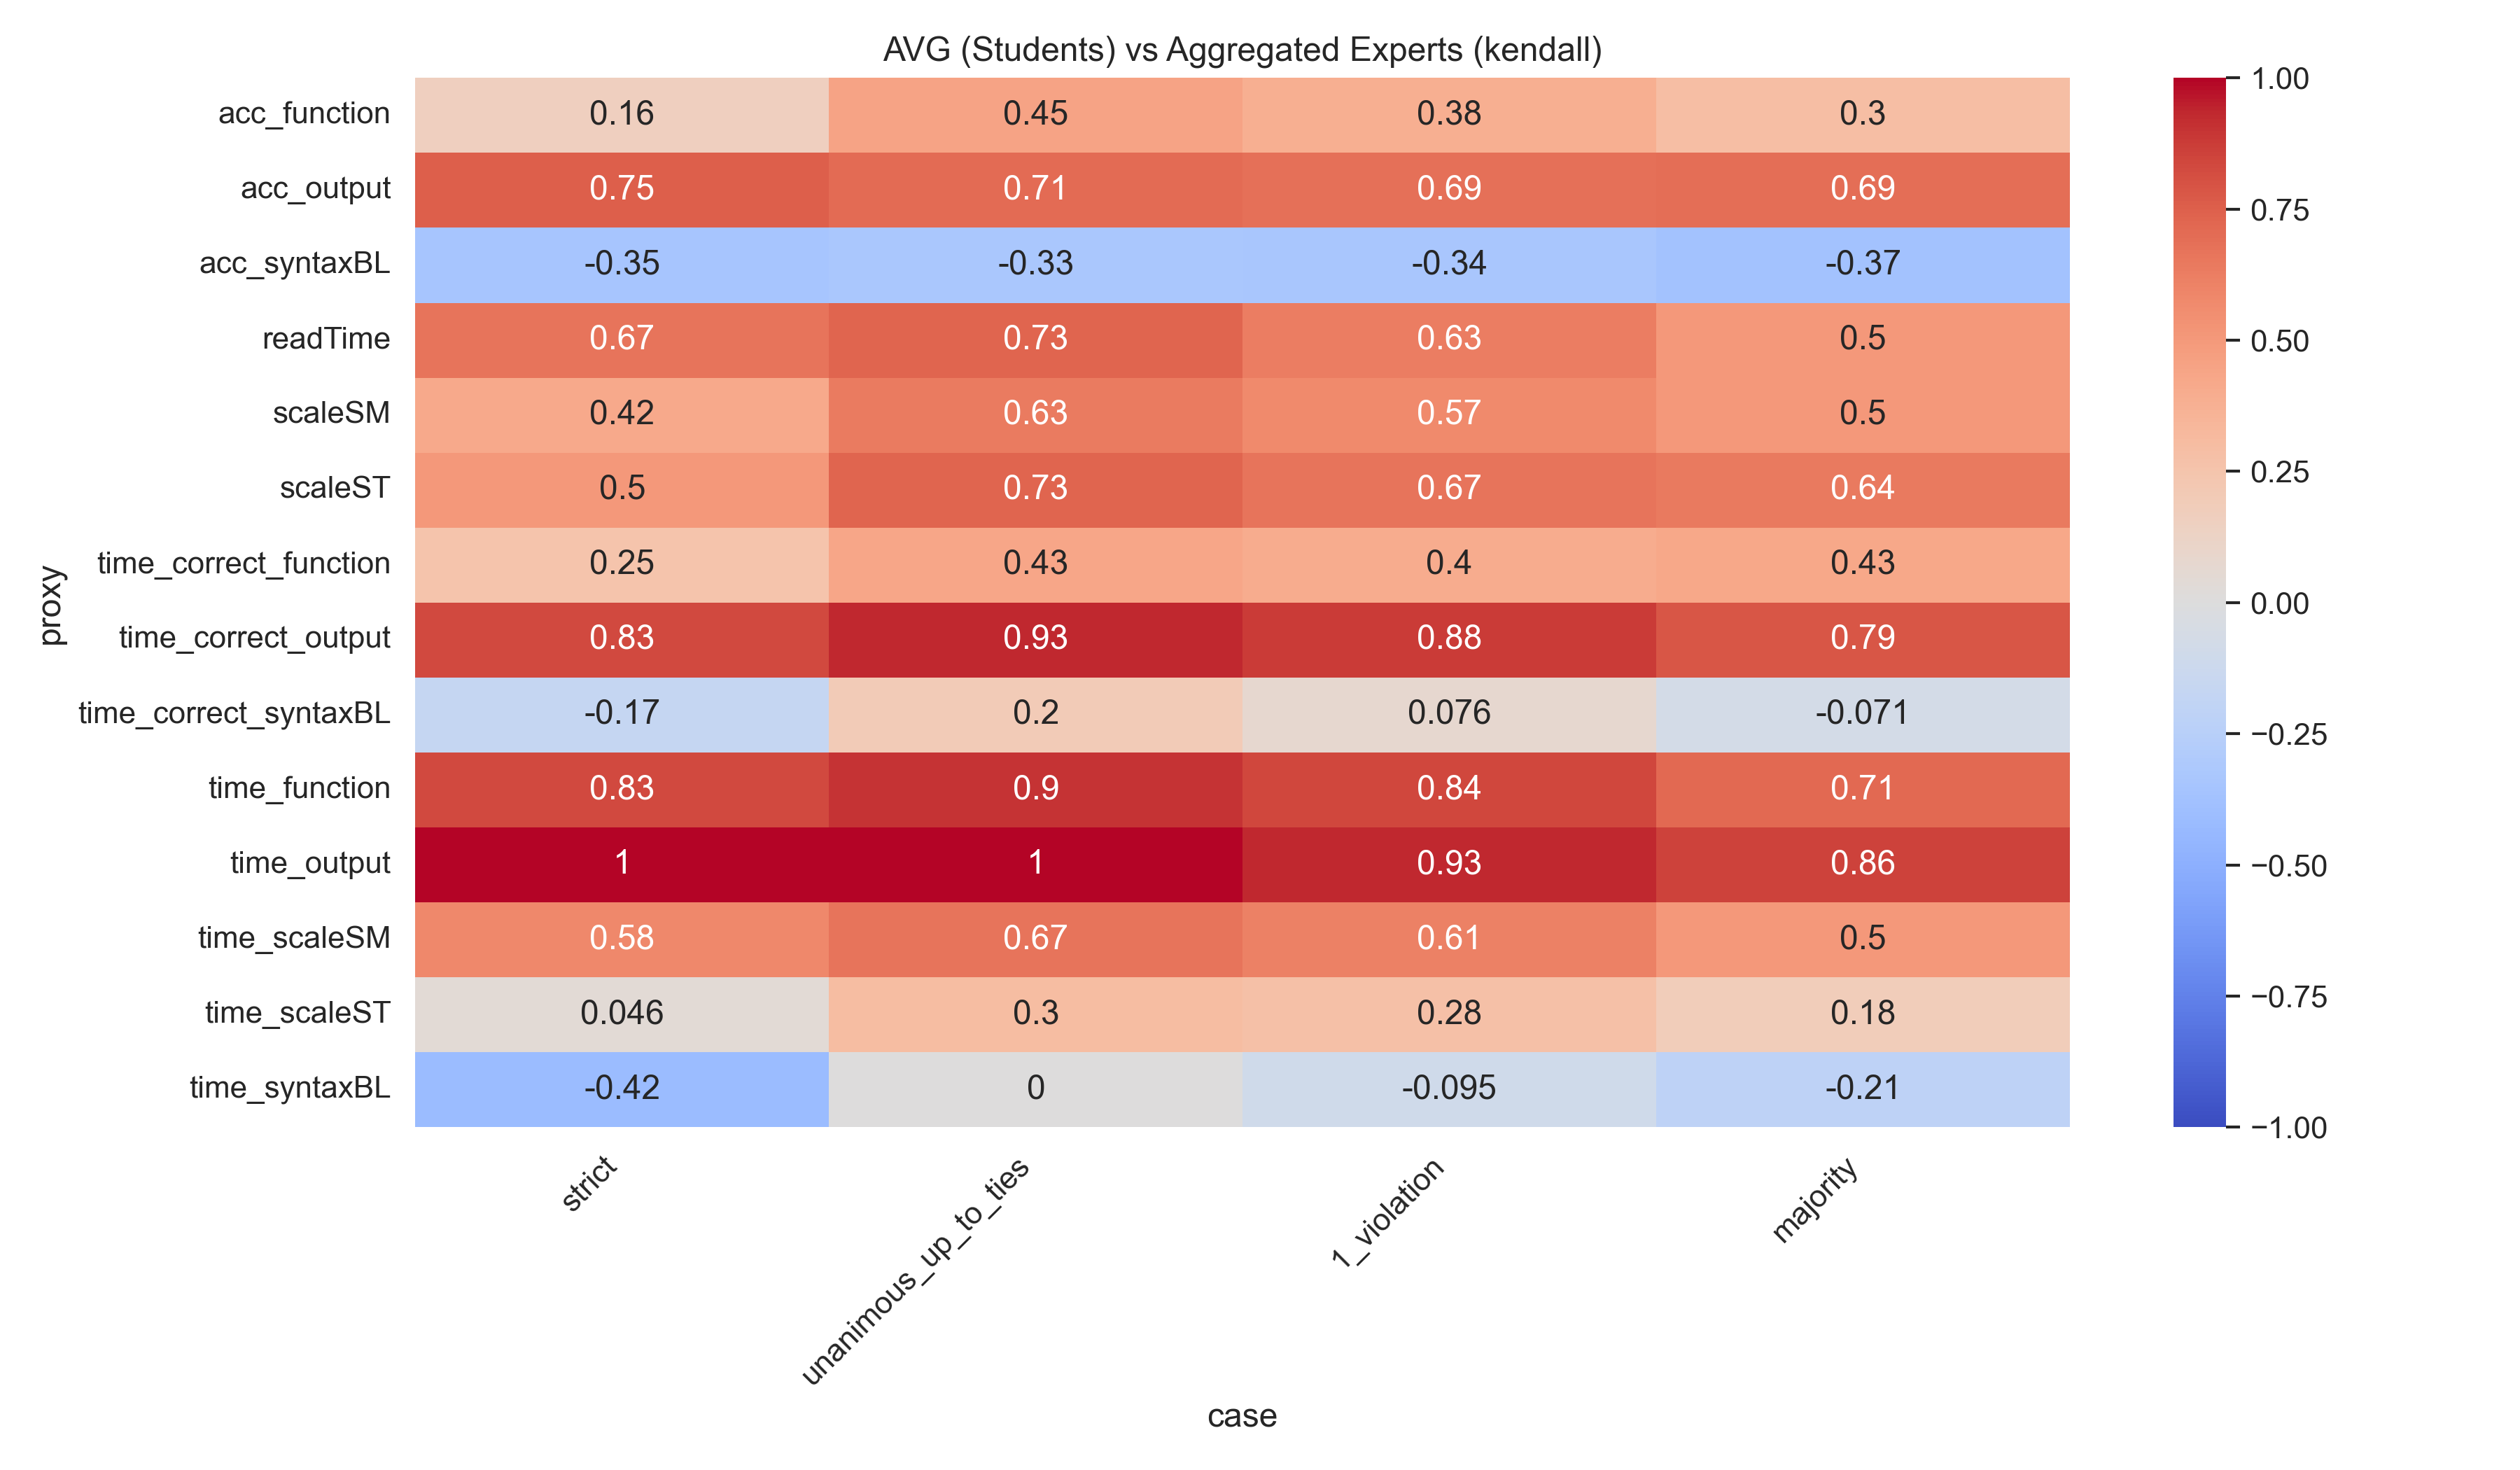
\includegraphics[width=0.9\linewidth]{figs/heatmap_agg_vs_agg_kendall.png}
    \caption{Correlation between aggregated student proxies and expert rankings across different expert aggregation strategies (Kendall).}
    \label{fig:heatmap_agg_vs_agg_kendall}
\end{figure}

\begin{figure}[t]
    \centering
    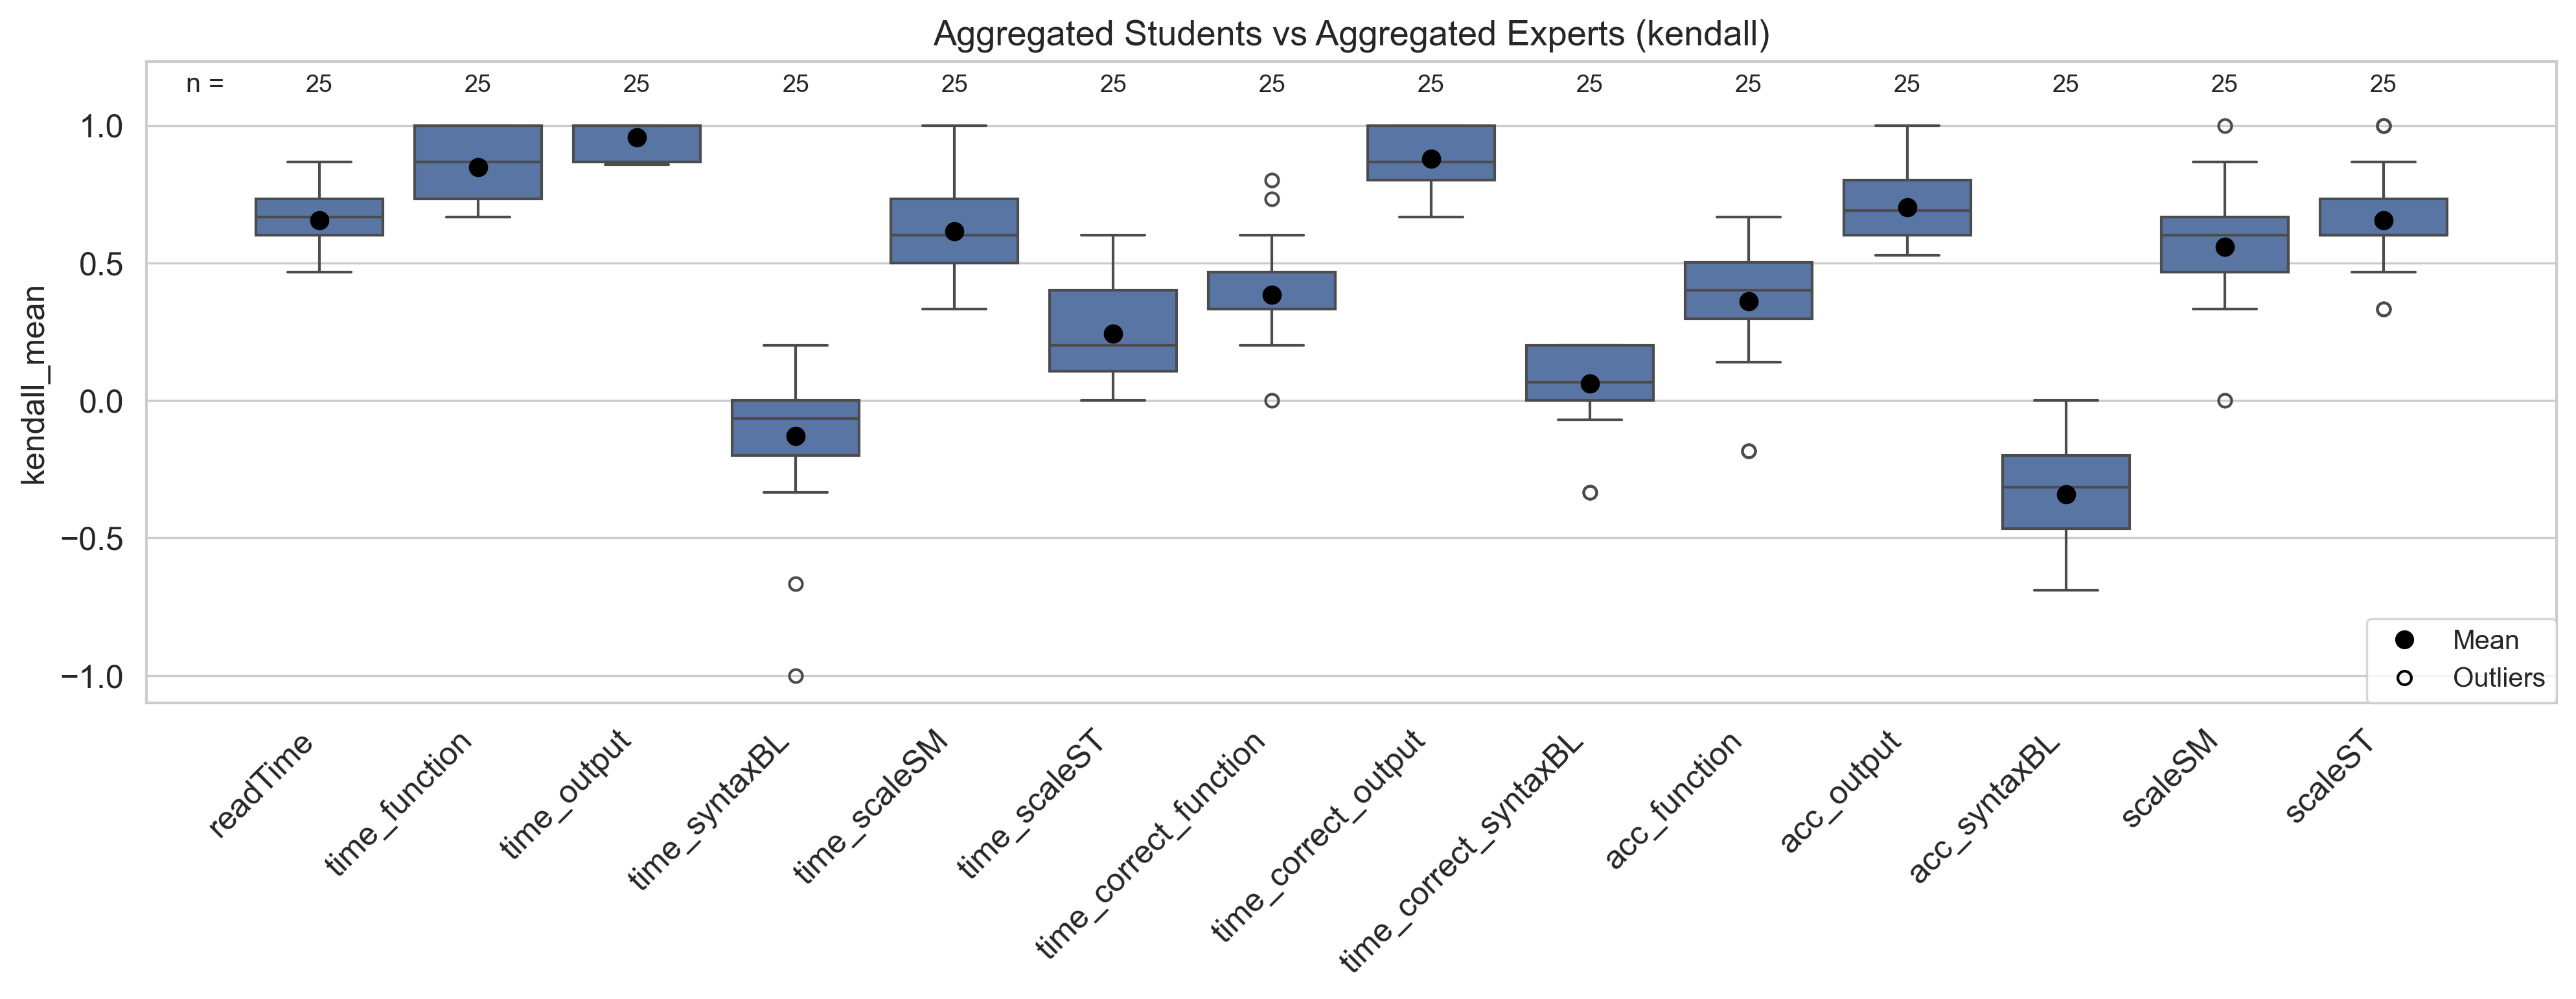
\includegraphics[width=0.9\linewidth]{figs/box_agg_vs_agg_kendall.png}
    \caption{Distribution of correlations between aggregated student proxies and expert rankings across aggregation strategies (Kendall).}
    \label{fig:box_agg_vs_agg_kendall}
\end{figure}

Figures~\ref{fig:heatmap_agg_vs_agg_kendall} and~\ref{fig:box_agg_vs_agg_kendall} show results across different expert aggregation strategies. While absolute correlation values vary, the relative ranking of proxies remains stable across aggregation methods.


% =====================================================
\subsection{No Aggregation in Expert Side}
\label{app:no-aggregation}
% =====================================================

\begin{figure}[t]
    \centering
    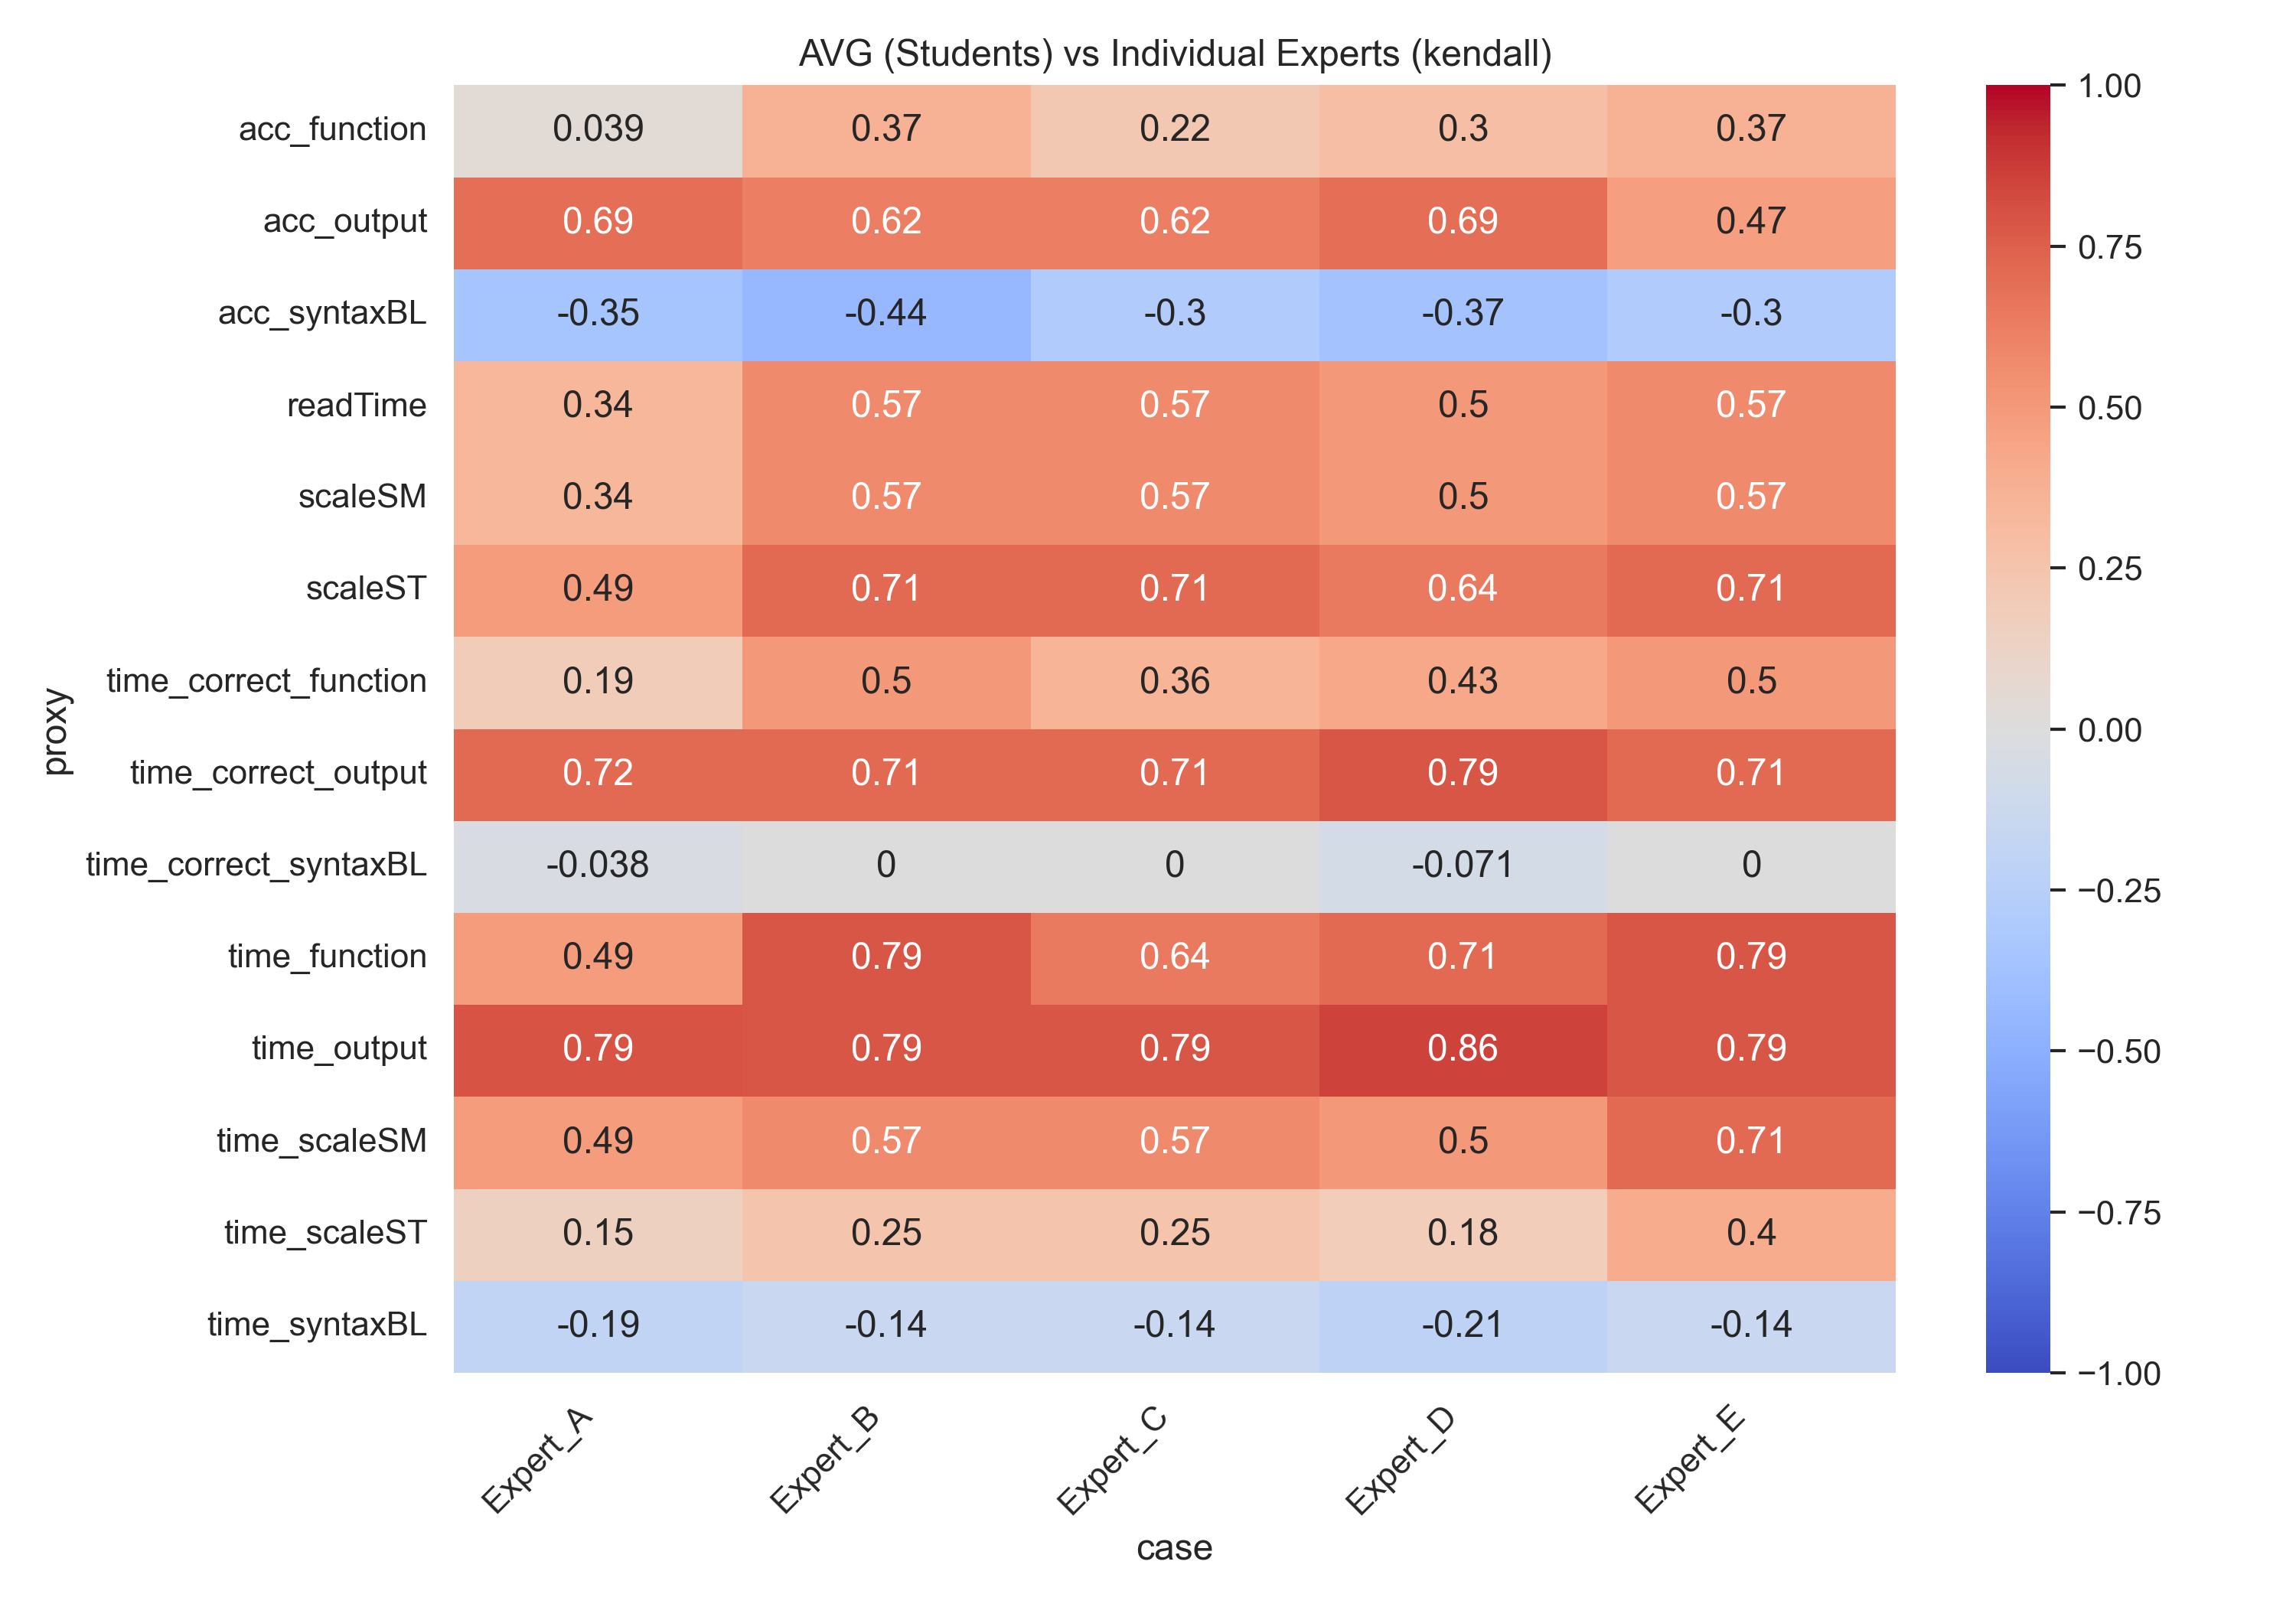
\includegraphics[width=0.9\linewidth]{figs/heatmap_avg_vs_expert_kendall.png}
    \caption{Correlation between aggregated student proxies and individual expert rankings (Kendall).}
    \label{fig:heatmap_avg_vs_expert_kendall}
\end{figure}

\begin{figure}[t]
    \centering
    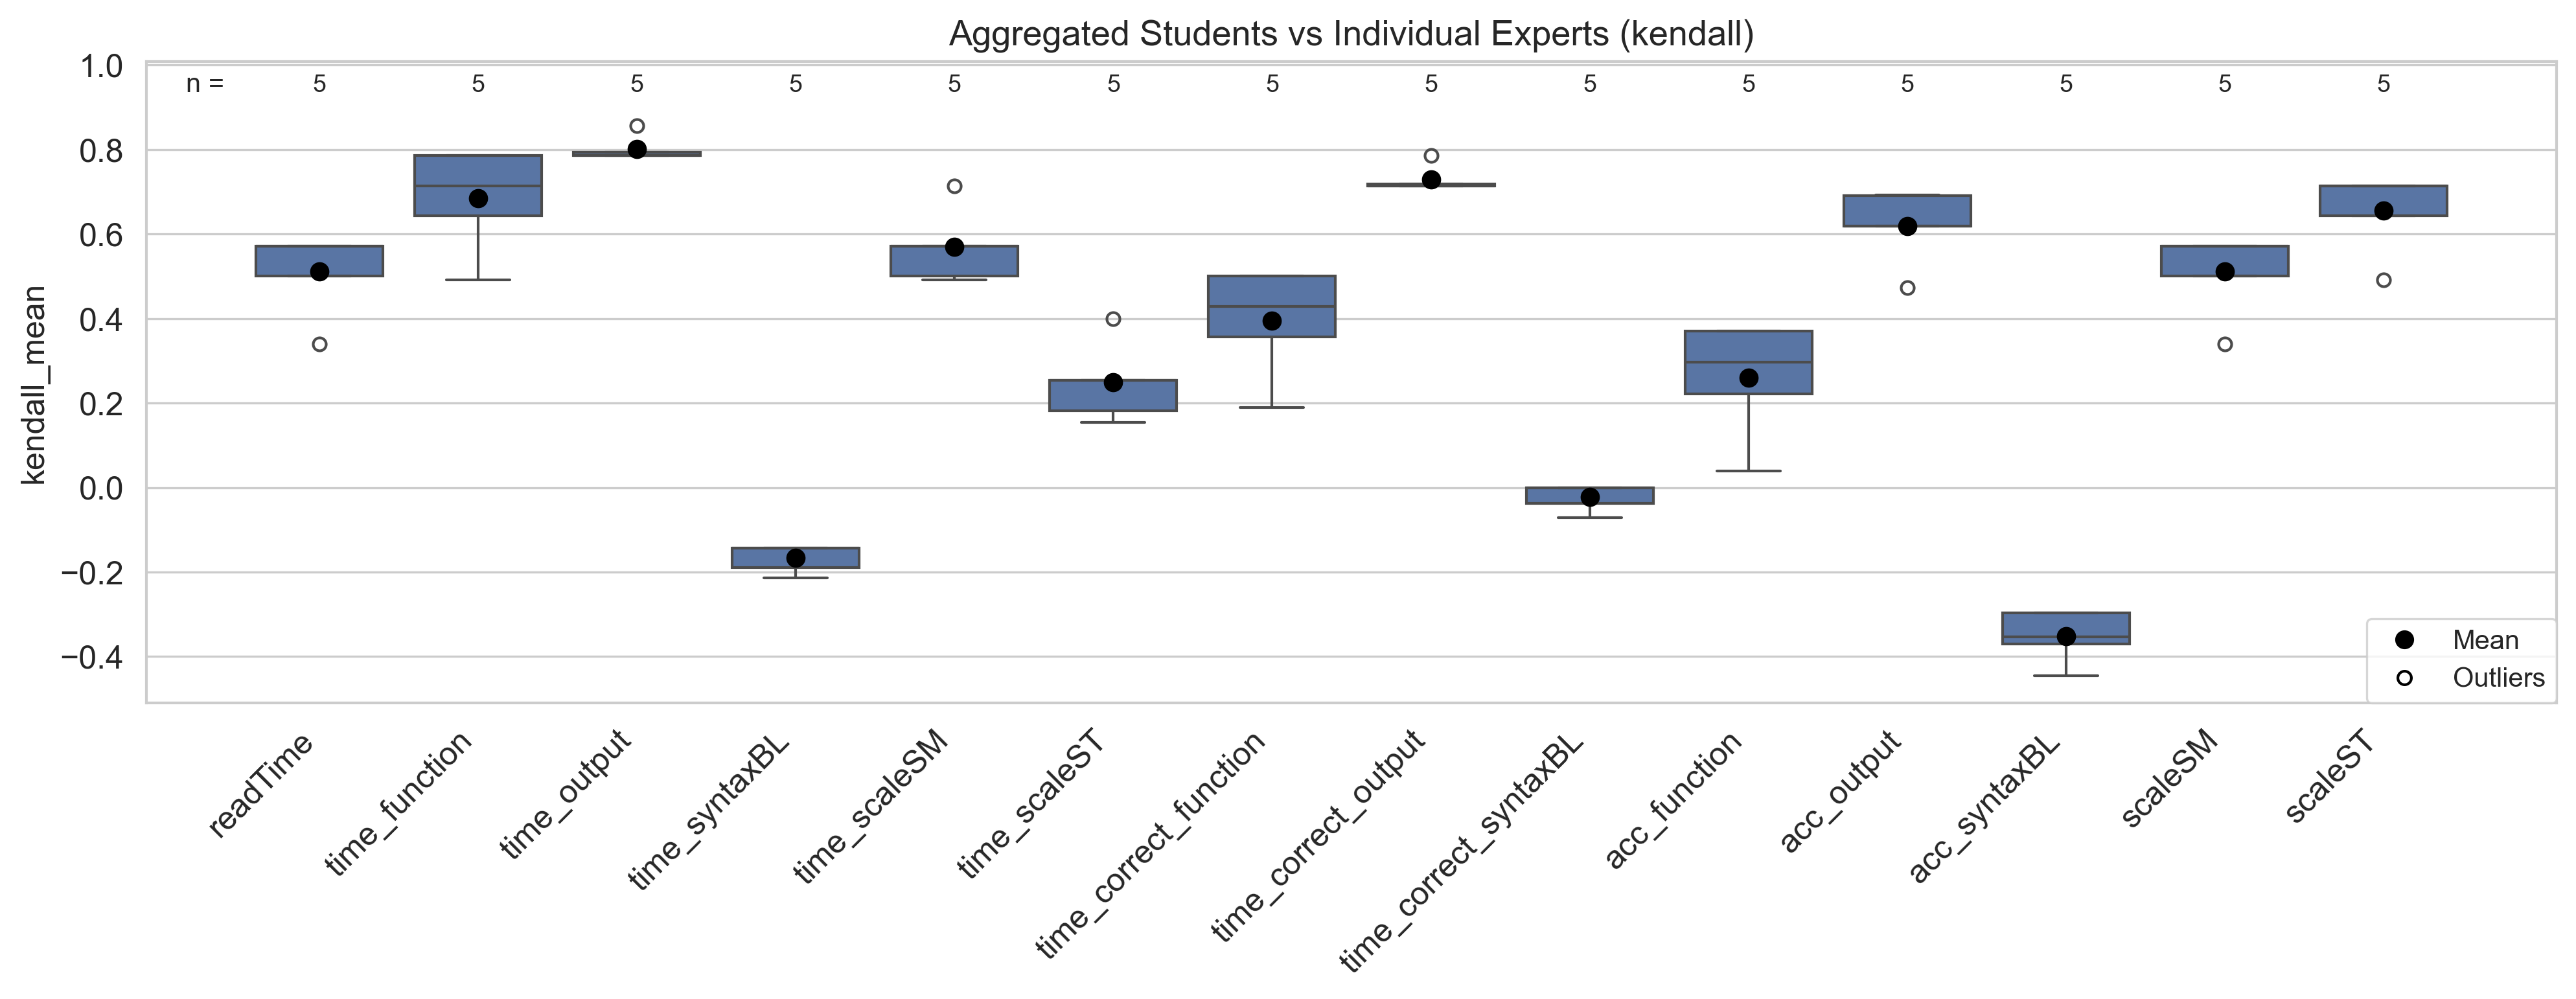
\includegraphics[width=0.9\linewidth]{figs/box_avg_vs_expert_kendall.png}
    \caption{Distribution of correlations between aggregated student proxies and individual expert rankings (Kendall).}
    \label{fig:box_avg_vs_expert_kendall}
\end{figure}

Figures~\ref{fig:heatmap_avg_vs_expert_kendall} and~\ref{fig:box_avg_vs_expert_kendall} compare aggregated student proxies against individual experts. The overall trends remain consistent, indicating that the results are not driven by a specific expert.

% =====================================================
\subsection{No Aggregation in Student Side (vs Aggregated Experts)}
\label{app:student-no-agg}
% =====================================================

\begin{figure}[t]
    \centering
    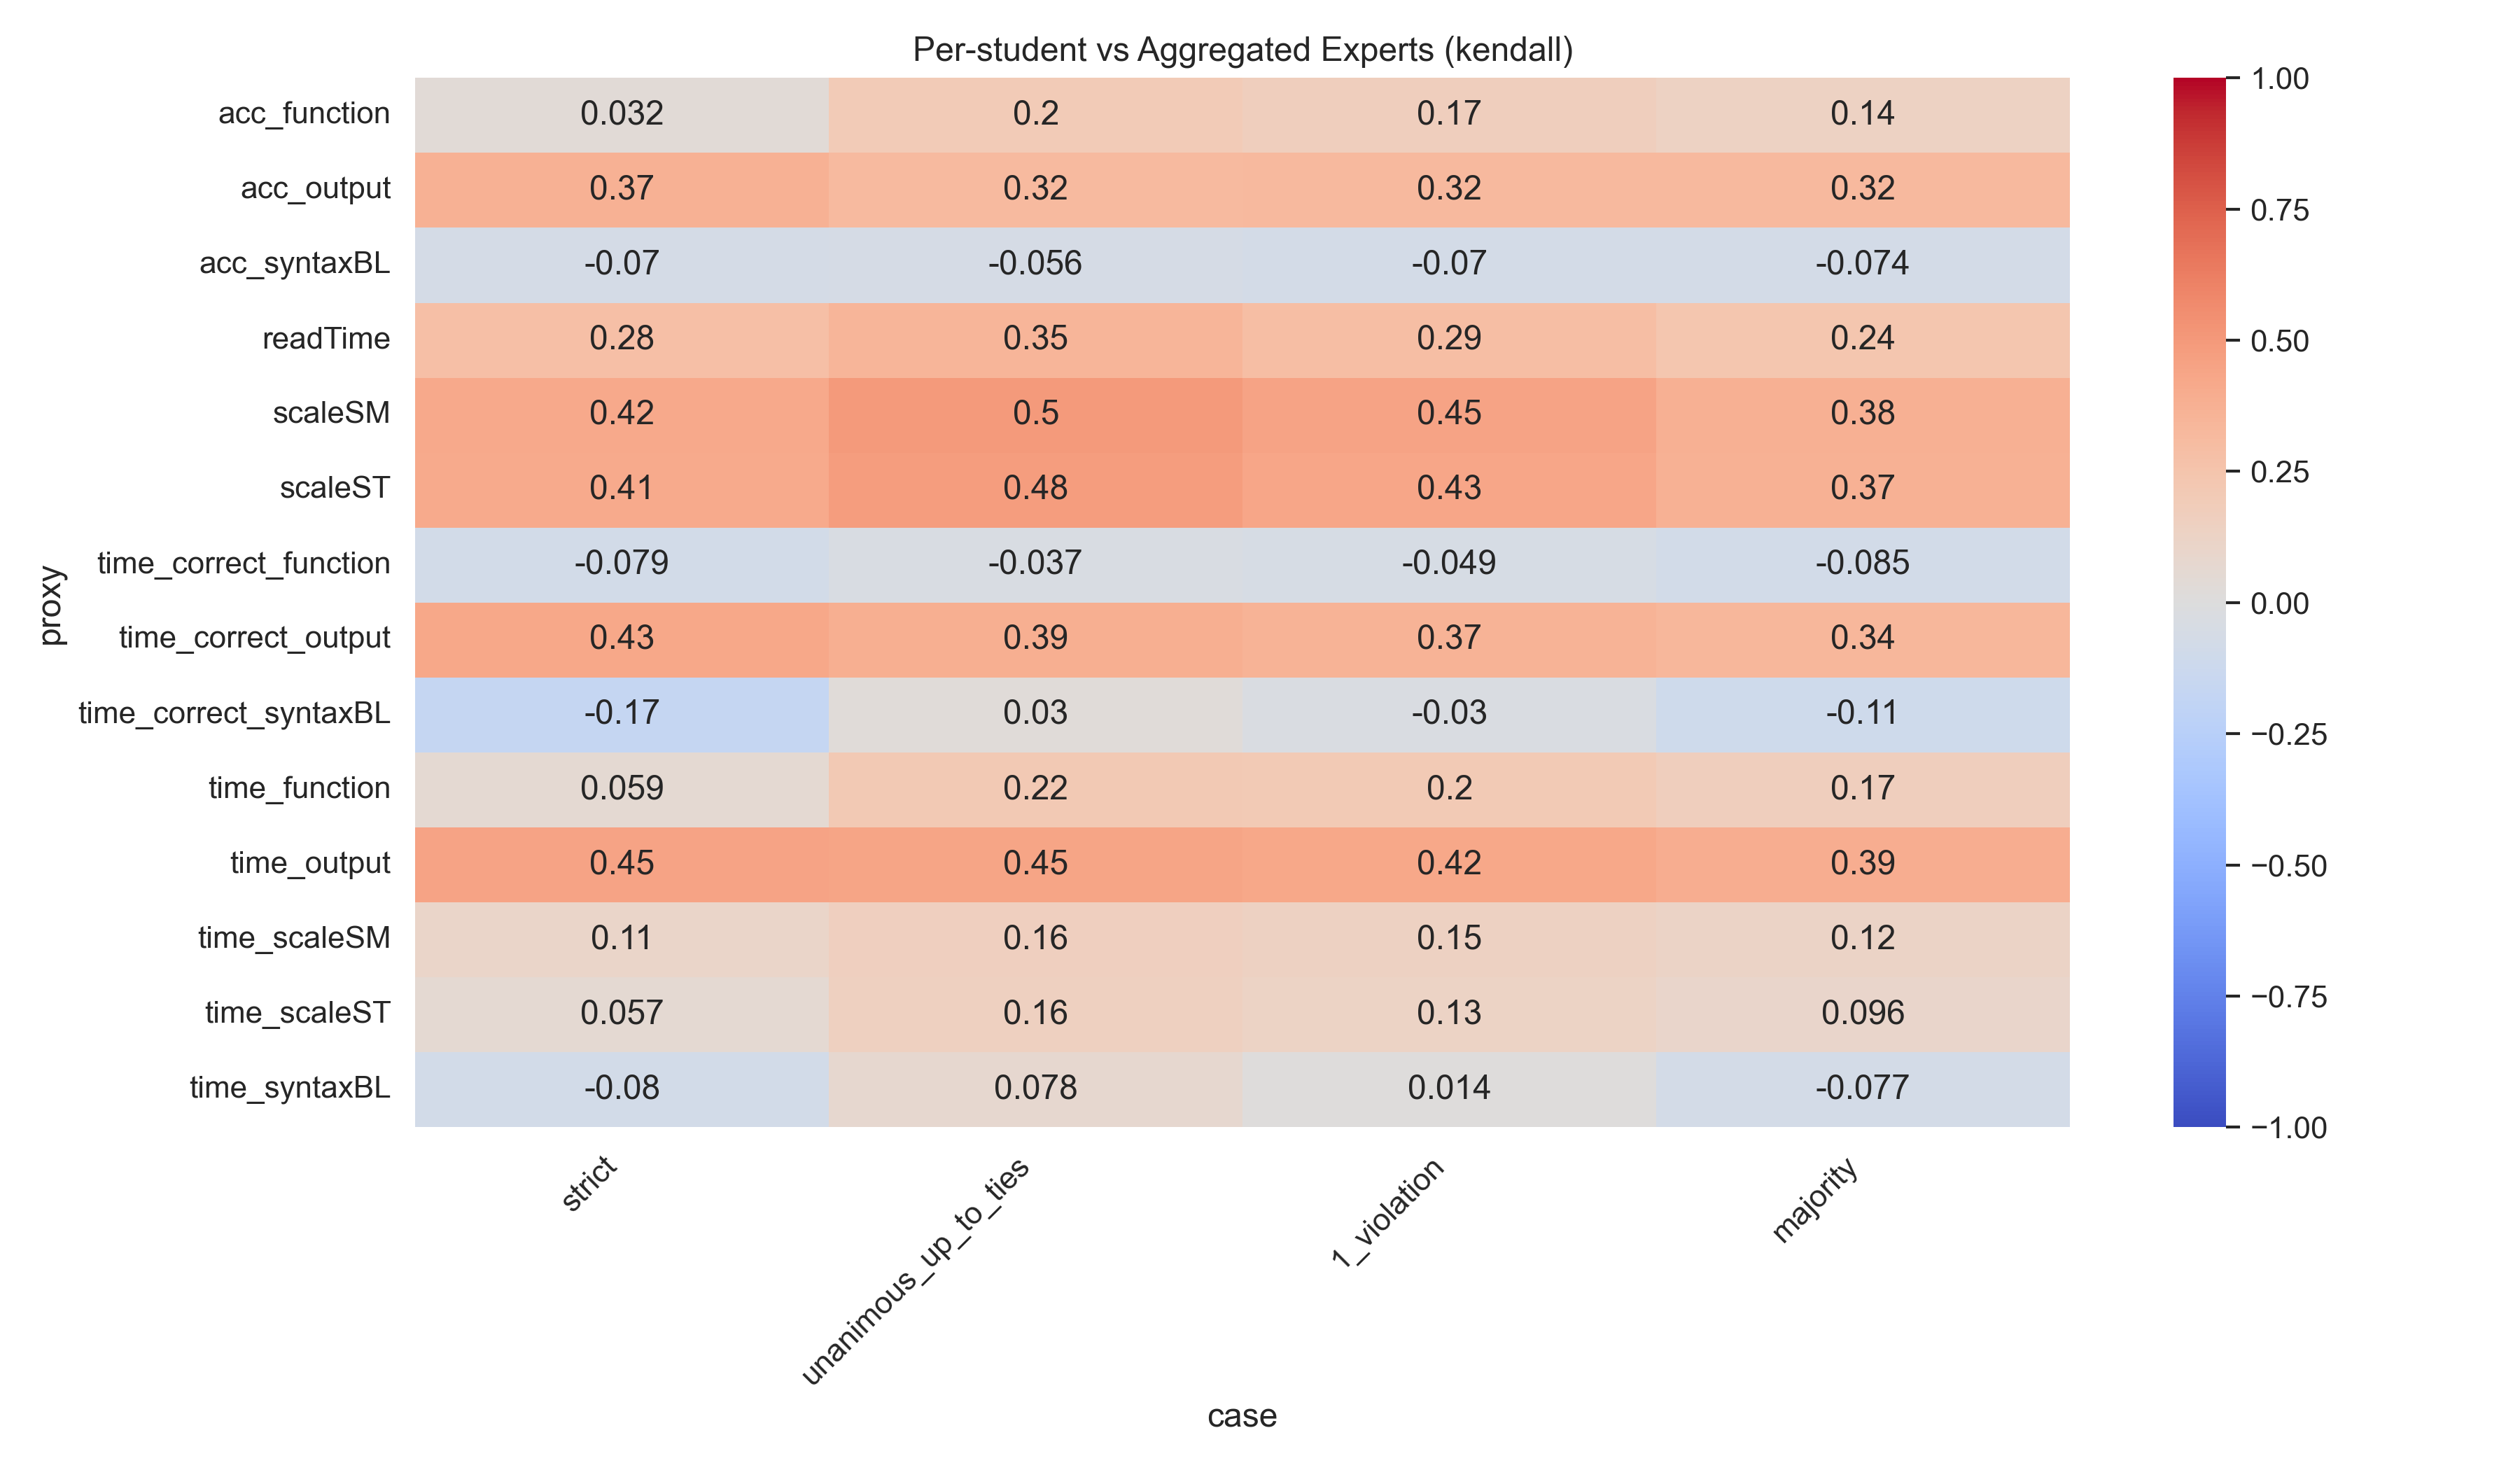
\includegraphics[width=0.9\linewidth]{figs/heatmap_perstudent_vs_aggexpert_kendall.png}
    \caption{Correlation between per-student proxy rankings and aggregated expert rankings (Kendall).}
    \label{fig:heatmap_perstudent_vs_agg_kendall}
\end{figure}

\begin{figure}[t]
    \centering
    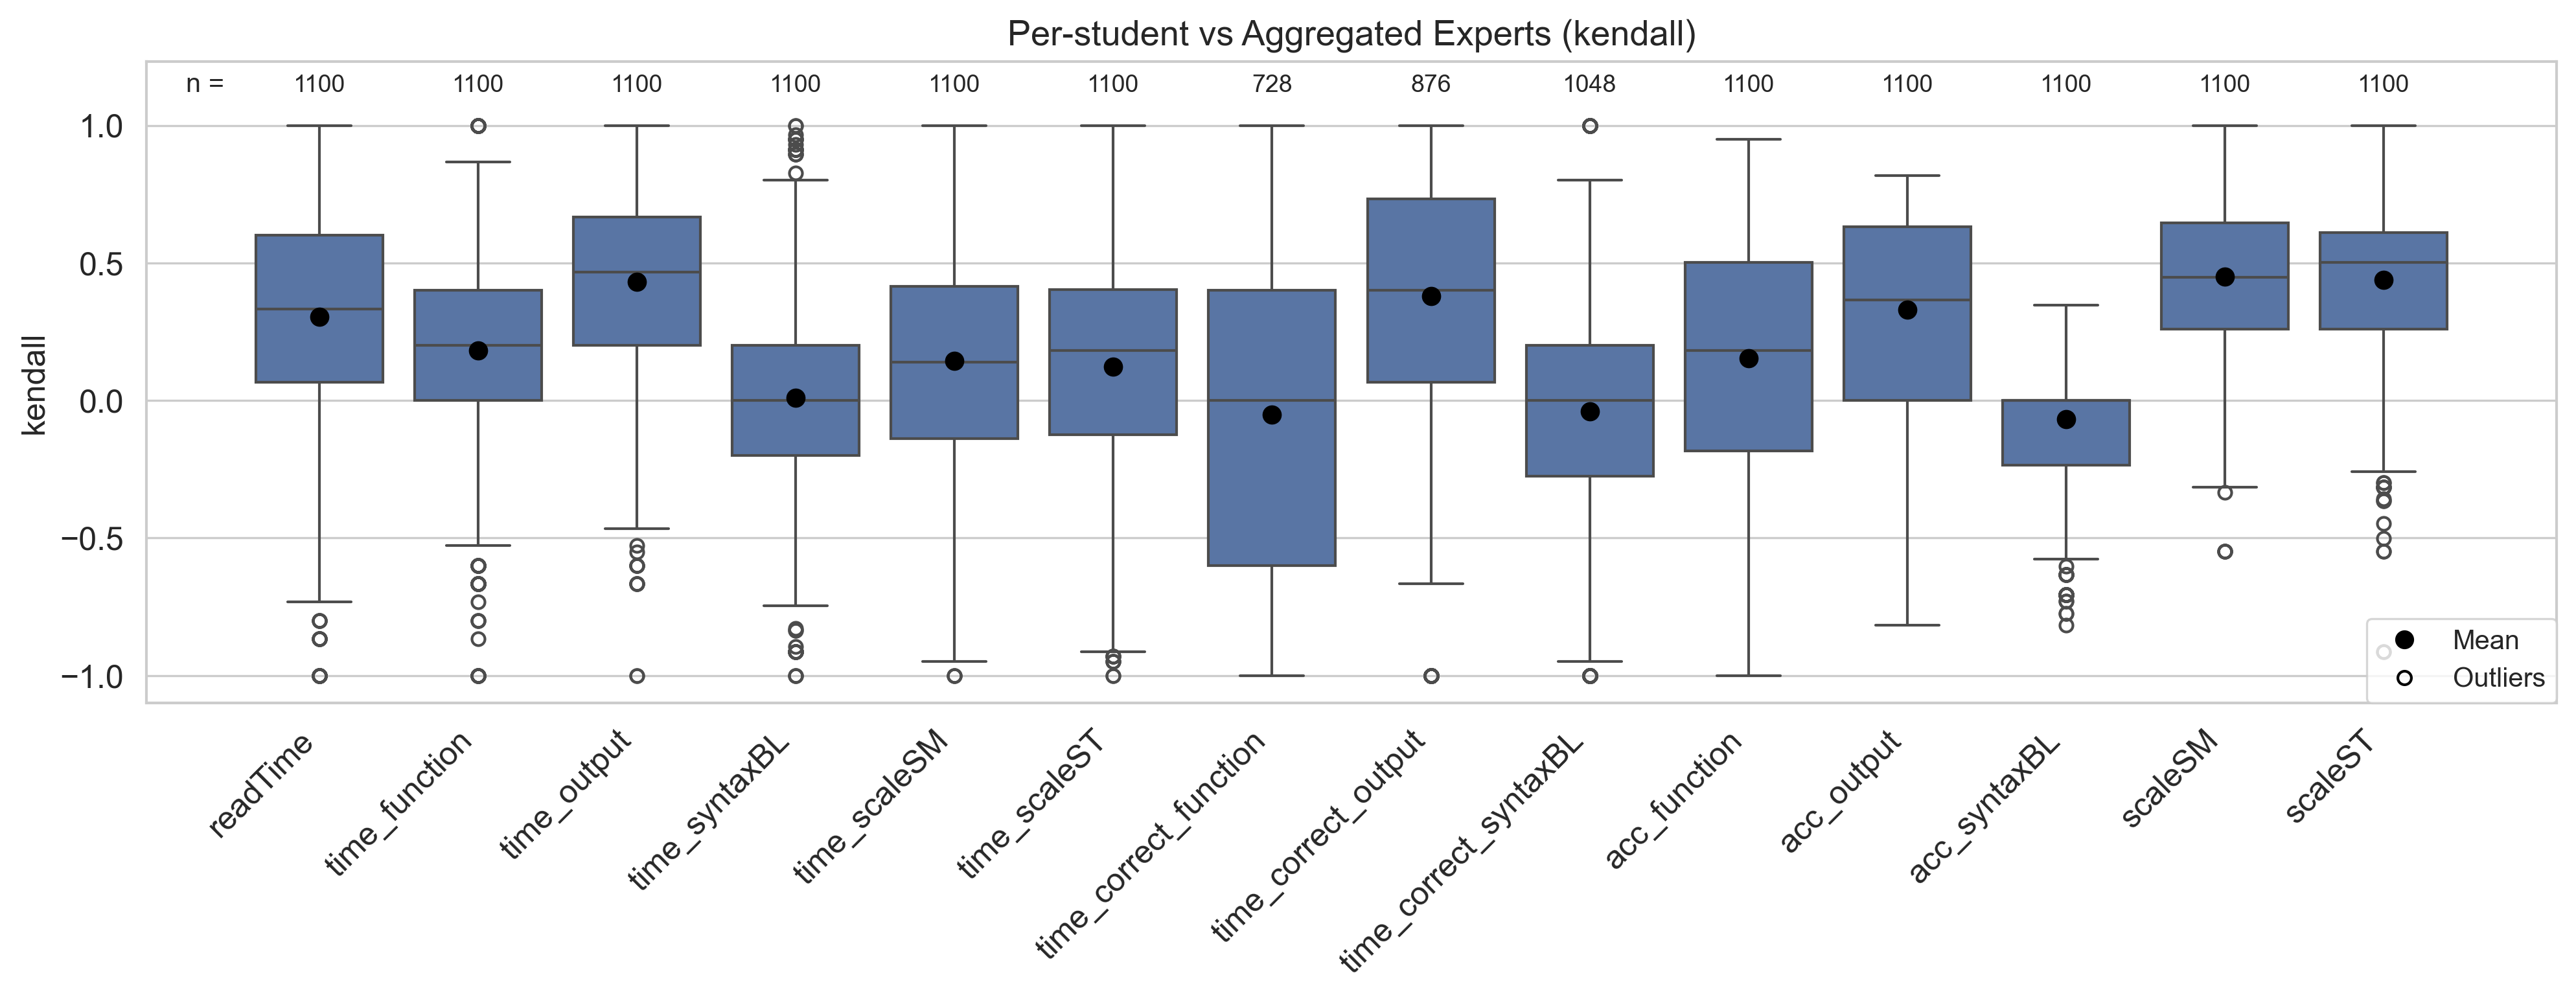
\includegraphics[width=0.9\linewidth]{figs/box_perstudent_vs_aggexpert_kendall.png}
    \caption{Distribution of correlations between per-student proxy rankings and aggregated expert rankings (Kendall).}
    \label{fig:box_perstudent_vs_agg_kendall}
\end{figure}

Figures~\ref{fig:heatmap_perstudent_vs_agg_kendall} and~\ref{fig:box_perstudent_vs_agg_kendall} show results without aggregating student data. The distributions exhibit higher variability, reflecting noise at the individual level.


% =====================================================
\subsection{No Aggregation in Both Sides}
\label{app:no-agg-at-all}
% =====================================================

\begin{figure}[t]
    \centering
    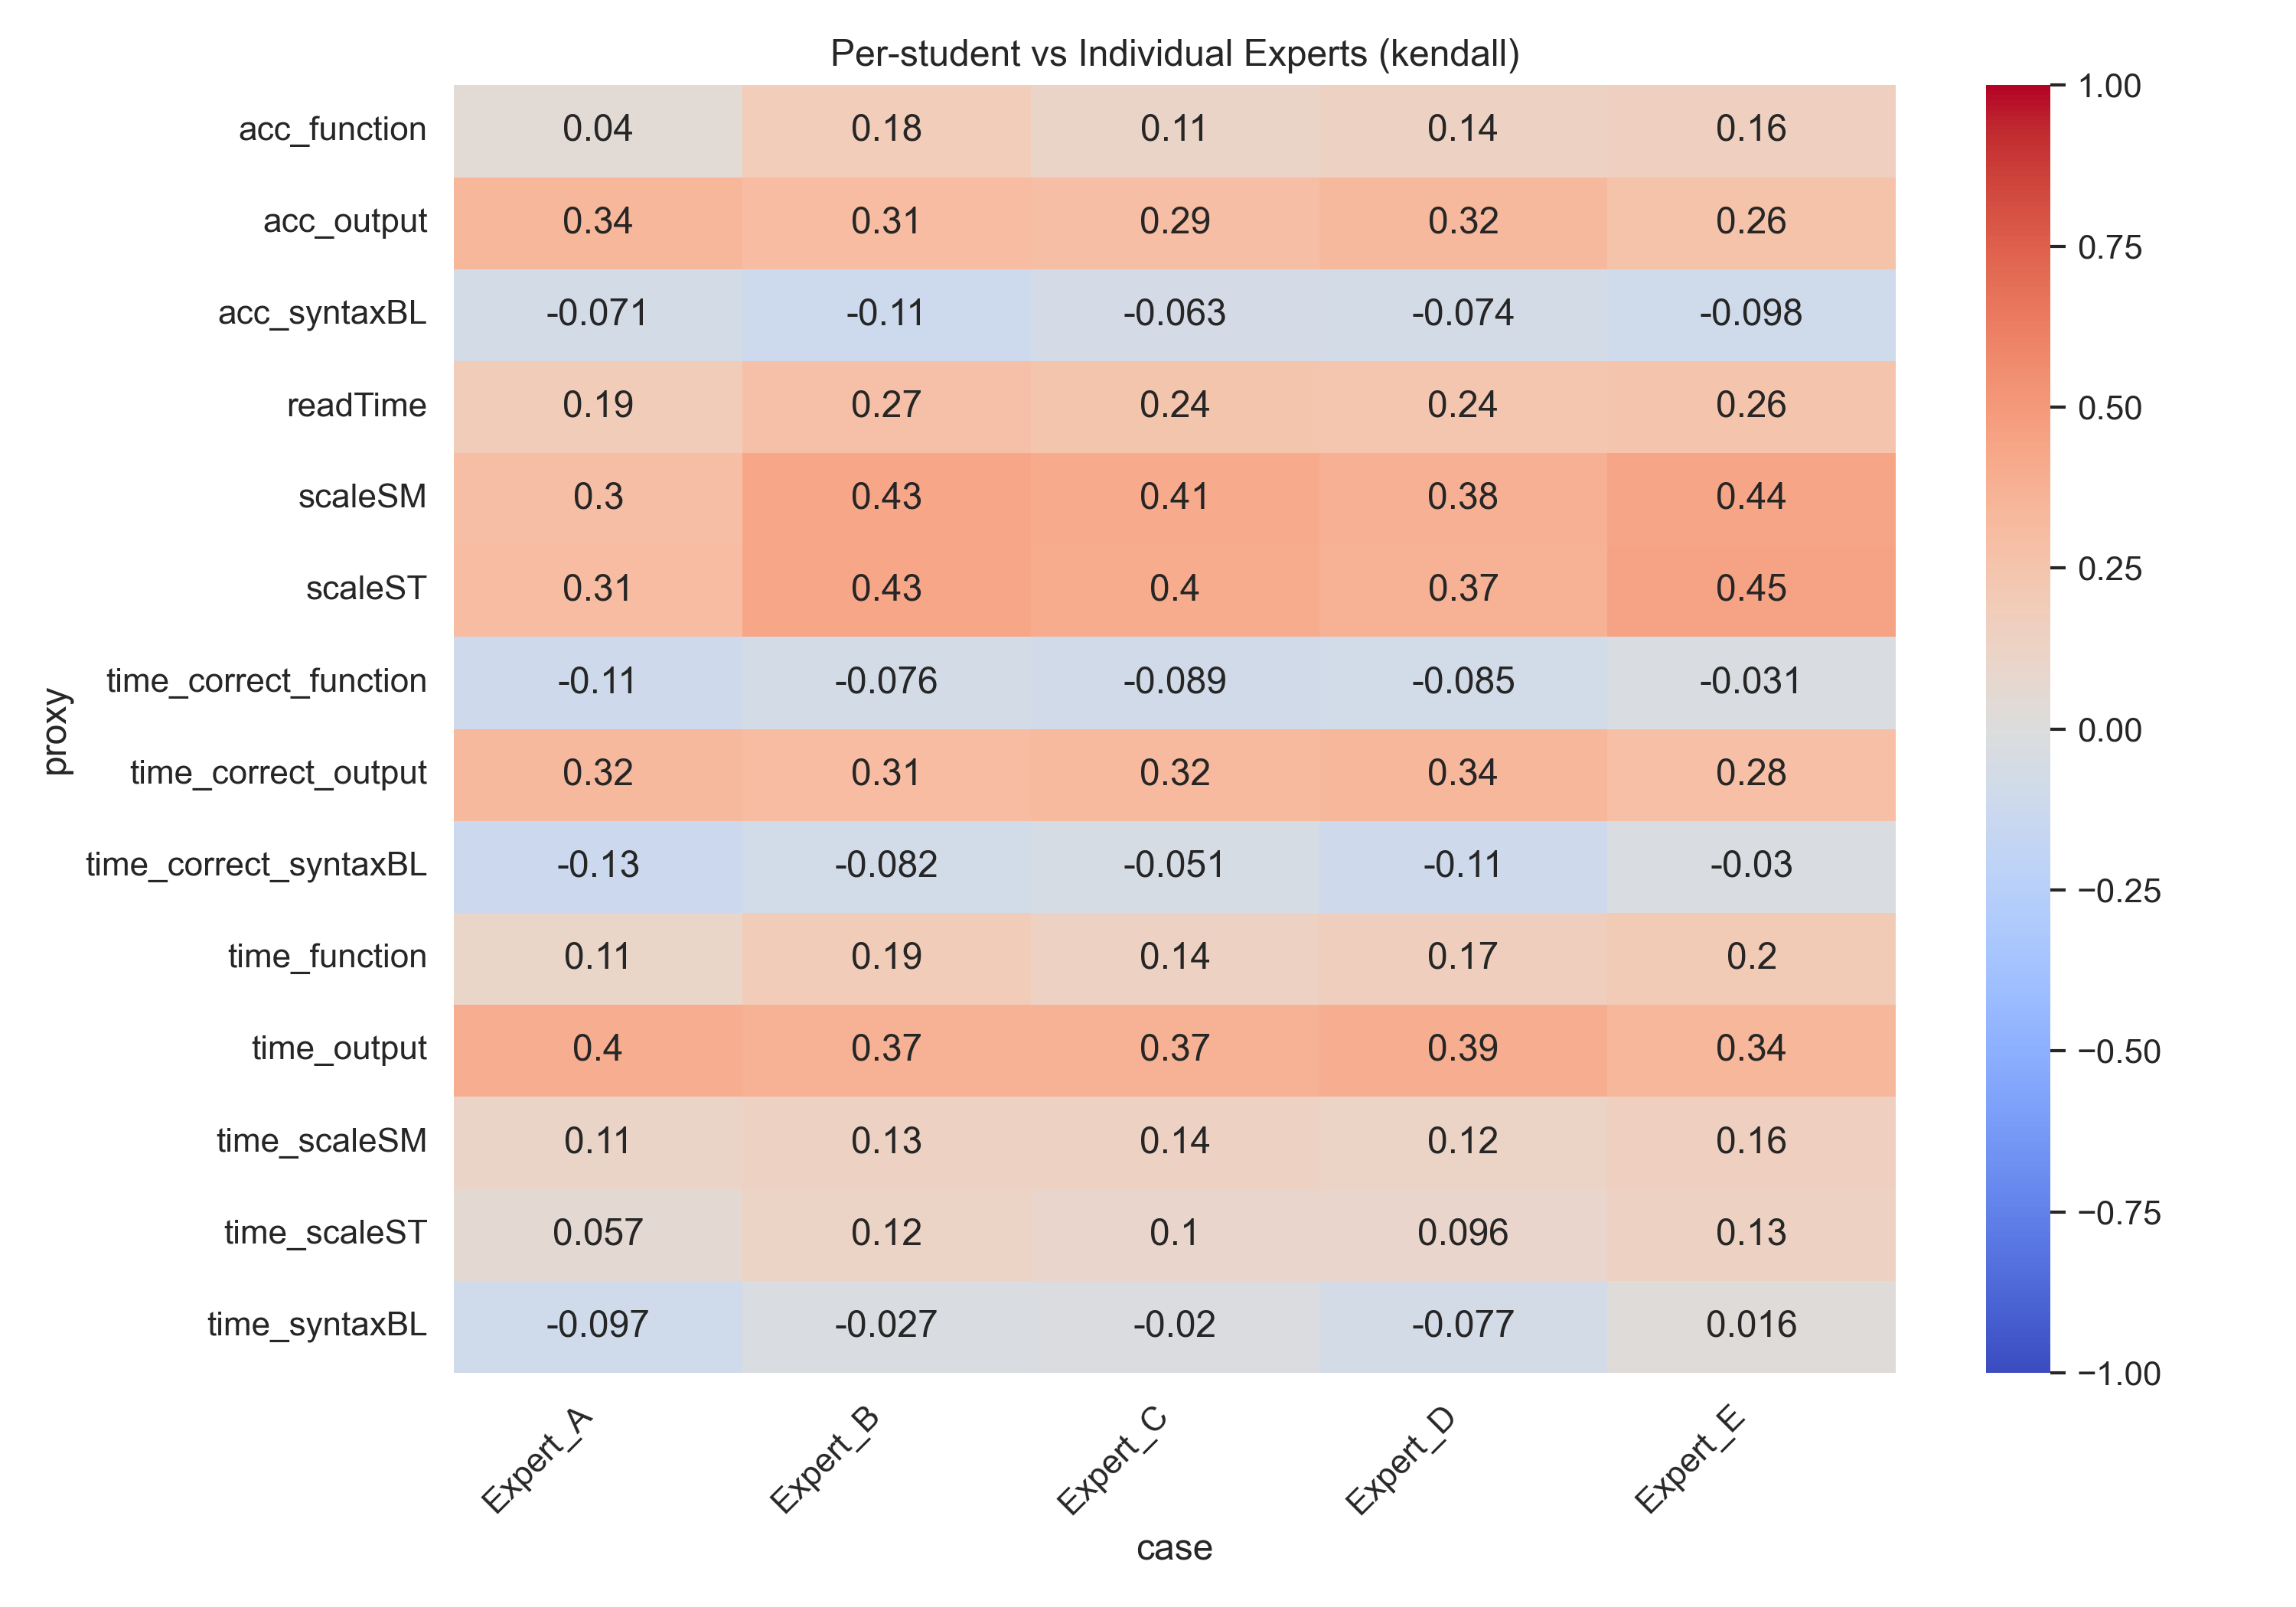
\includegraphics[width=0.9\linewidth]{figs/heatmap_perstudent_vs_expert_kendall.png}
    \caption{Correlation between per-student proxy rankings and individual expert rankings (Kendall).}
    \label{fig:heatmap_perstudent_vs_expert_kendall}
\end{figure}

\begin{figure}[t]
    \centering
    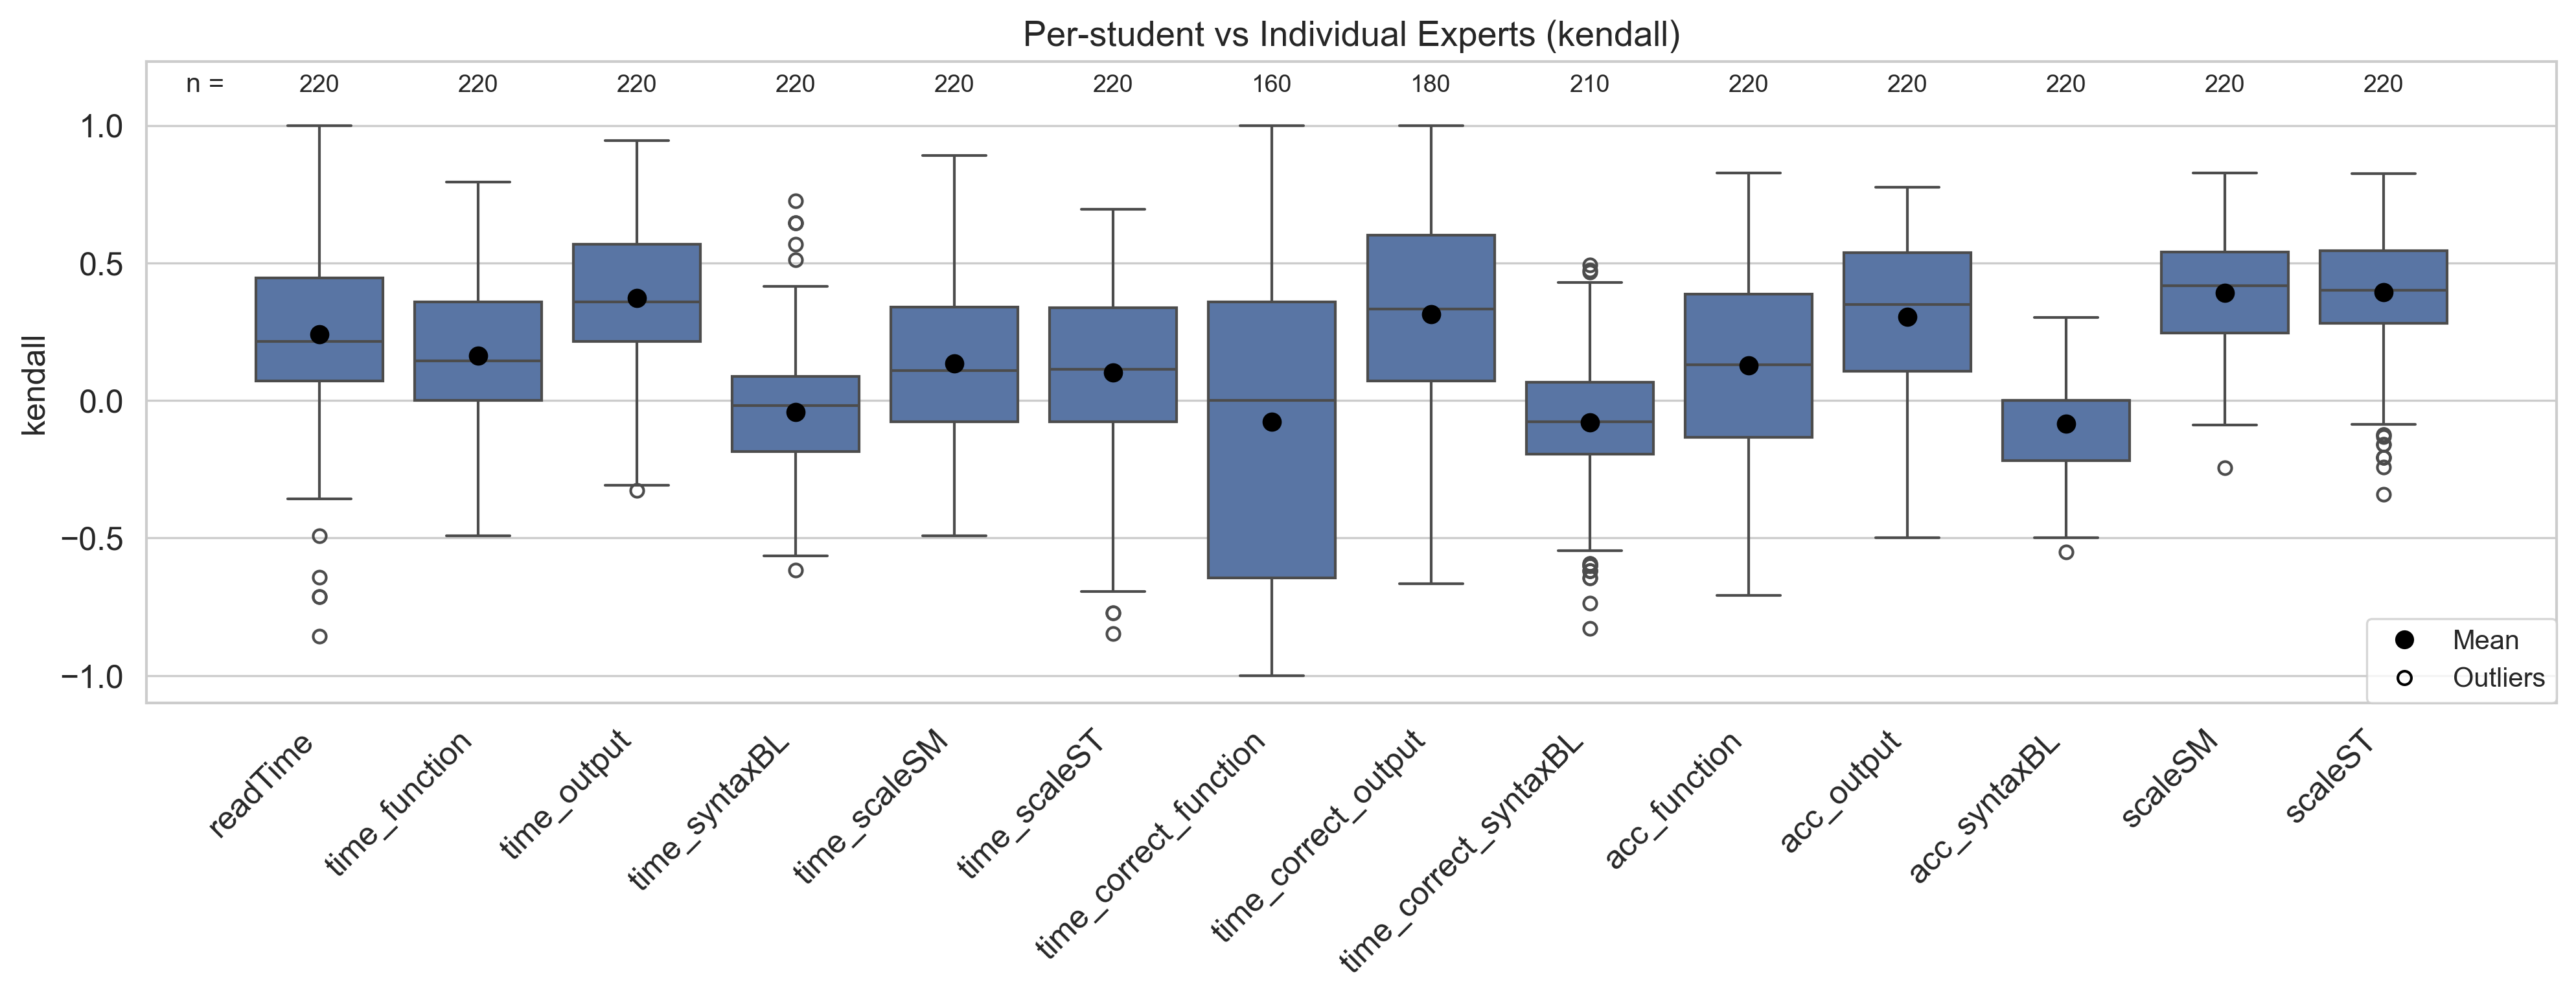
\includegraphics[width=0.9\linewidth]{figs/box_perstudent_vs_expert_kendall.png}
    \caption{Distribution of correlations between per-student proxy rankings and individual expert rankings (Kendall).}
    \label{fig:box_perstudent_vs_expert_kendall}
\end{figure}

Figures~\ref{fig:heatmap_perstudent_vs_expert_kendall} and~\ref{fig:box_perstudent_vs_expert_kendall} present the fully unaggregated setting. Correlations are more dispersed, but the overall ordering of proxies remains consistent.

\subsection{Impact of Student Characteristics and Fatigue on Code Comprehension Performance}
\label{app:results-background}

\subsubsection{Overview}

We analyze whether student background characteristics and task order influence code comprehension performance in our study. Specifically, we investigate whether self-reported programming experience, object-oriented programming knowledge, background knowledge, and fatigue affect multiple comprehension proxies. Rather than aggregating across question types, we analyze accuracy and time separately for the function, output, and syntax tasks. We also analyze snippet reading time and total time spent on each snippet.

Participants solved eight code comprehension tasks presented in randomized order. For each task, participants first read a code snippet and then answered three comprehension questions: one function question, one output question, and one syntax question. The dataset therefore contains repeated measurements for each participant across multiple snippets and question types.

\subsubsection{Data Structure}

The dataset contains repeated observations for each participant. Each participant solved eight code comprehension tasks, and each task includes three comprehension questions. Therefore, the data can be represented at two levels relevant to the present analysis:

\begin{itemize}

\item \textbf{Question level}: Each observation corresponds to a single comprehension question (function, output, or syntax). This dataset contains up to $44 \times 8 \times 3 = 1056$ observations.

\item \textbf{Snippet level}: Each observation corresponds to a participant--snippet pair. This dataset contains up to $44 \times 8 = 352$ observations.

\end{itemize}

Different statistical models are applied depending on the level at which the outcome variable is defined.

\subsubsection{Measured Outcomes}

We consider the following outcome variables:

\begin{itemize}

\item \textbf{\emph{acc\_function}, \emph{acc\_output}, and \emph{acc\_syntaxBL}}: Binary variables indicating whether the corresponding question was answered correctly. For function questions, correctness is defined using the grading threshold adopted in our study; output and syntax questions use their existing binary correctness labels.

\item \textbf{\emph{time\_function}, \emph{time\_output}, and \emph{time\_syntaxBL}}: Raw time spent answering each question type.

\item \textbf{\emph{time\_correct\_function}, \emph{time\_correct\_output}, and\\
\emph{time\_correct\_syntaxBL}}: Raw time spent answering a question, restricted to cases in which the answer was correct.

\item \textbf{\emph{readTime}}: The time spent reading a snippet before answering questions.

\item \textbf{\emph{snippet\_total\_time}}: The total time spent on a snippet, defined as the sum of the reading time and the times spent answering the three comprehension questions.

\end{itemize}

\subsubsection{Predictor Variables}

We analyze the following participant-level predictors:

\begin{itemize}

\item \textbf{Programming Experience Relative to Peers}: A self-reported measure of programming ability compared to classmates.

\item \textbf{Java Experience (Years)}

\item \textbf{Object-Oriented Experience}: Self-rated experience with object-oriented programming.

\item \textbf{Programming Experience Score}

\item \textbf{Background Knowledge}: A knowledge score derived from responses to eleven multiple-choice familiarity questions about snippets.

\item \textbf{Fatigue}: The position of the snippet in the experiment (1--8), representing task order.

\end{itemize}

All participant-level background predictors were standardized to $z$-scores prior to modeling. Fatigue was operationalized directly as snippet position.

\subsubsection{Statistical Models}

Because participants completed multiple tasks, observations are not independent. We therefore use statistical models that account for repeated measurements.

\paragraph{Accuracy Models}

Accuracy is measured at the question level and is a binary variable indicating whether a comprehension question was answered correctly. We analyze each accuracy proxy separately using logistic regression estimated with clustered standard errors:

\[
\text{accuracy}_{i,j,k} \sim \beta_0 + \beta_1 \text{predictor}_i + \gamma_j
\]

where $i$ indexes participants, $j$ indexes snippets, and $k$ indexes question type. The model includes fixed effects for snippet identity ($\gamma_j$) to control for differences in snippet difficulty, and standard errors are clustered by participant to account for repeated observations.

\paragraph{Time Models}

Question-level time proxies, snippet reading time, and snippet total time are continuous outcomes. We analyze them using linear mixed-effects models:

\[
\text{time}_{i,j,k} \sim \beta_0 + \beta_1 \text{predictor}_i + \gamma_j + u_i
\]

where $u_i$ is a random intercept for participant $i$, capturing individual differences in baseline speed.

\subsubsection{Results and Interpretation}

\Cref{tab:student_factors_final} summarizes the estimated coefficients, standard errors, p-values, and 95\% confidence intervals. Each row in \cref{tab:student_factors_final} corresponds to a separate regression model estimating the effect of a single predictor variable on one comprehension proxy.

For example, the row \emph{Programming Experience Relative to Peers -- acc\_function} estimates the effect of peer-relative programming experience on function-question accuracy, while the row \emph{Fatigue -- time\_output} estimates the effect of snippet order on the time spent answering output questions.


\begin{table}[t]
\scriptsize
\centering
\caption{Impact of participant characteristics and fatigue on comprehension proxies. The table reports results for all estimated models. Coefficients are reported with 95\% confidence intervals. Significant results ($p < 0.05$) are shown in bold.}
\label{tab:student_factors_final}
\begin{tabular}{llllrrr}
\toprule
Analysis & Outcome & Predictor & $\beta$ & SE & $p$ & CI \\
\midrule

\multicolumn{7}{l}{\textbf{PRP}} \\
PRP & acc\_function & PRP & \textbf{0.33} & 0.15 & \textbf{0.024} & [0.04, 0.61] \\
PRP & acc\_output & PRP & \textbf{0.36} & 0.18 & \textbf{0.045} & [0.01, 0.71] \\
PRP & acc\_syntaxBL & PRP & -0.04 & 0.18 & 0.83 & [-0.39, 0.31] \\
PRP & time\_function & PRP & 5.99 & 9.60 & 0.53 & [-12.83, 24.82] \\
PRP & time\_output & PRP & -2.04 & 6.11 & 0.74 & [-14.02, 9.94] \\
PRP & time\_syntaxBL & PRP & -1.05 & 0.76 & 0.16 & [-2.53, 0.43] \\
PRP & time\_correct\_function & PRP & 2.92 & 7.69 & 0.70 & [-12.15, 17.99] \\
PRP & time\_correct\_output & PRP & -5.43 & 6.84 & 0.43 & [-18.84, 7.97] \\
PRP & time\_correct\_syntaxBL & PRP & -1.32 & 0.72 & 0.07 & [-2.73, 0.10] \\
PRP & readTime & PRP & -3.13 & 6.75 & 0.64 & [-16.36, 10.11] \\

\midrule

\multicolumn{7}{l}{\textbf{JavaExp}} \\
JavaExp & acc\_function & JavaExp & -0.12 & 0.18 & 0.51 & [-0.47, 0.24] \\
JavaExp & acc\_output & JavaExp & -0.10 & 0.16 & 0.54 & [-0.42, 0.22] \\
JavaExp & acc\_syntaxBL & JavaExp & -0.43 & 0.25 & 0.09 & [-0.91, 0.06] \\
JavaExp & time\_function & JavaExp & 11.82 & 9.48 & 0.21 & [-6.76, 30.39] \\
JavaExp & time\_output & JavaExp & 7.03 & 6.12 & 0.25 & [-4.97, 19.03] \\
JavaExp & time\_syntaxBL & JavaExp & 0.32 & 0.77 & 0.68 & [-1.20, 1.83] \\
JavaExp & time\_correct\_function & JavaExp & 7.20 & 8.28 & 0.38 & [-9.03, 23.43] \\
JavaExp & time\_correct\_output & JavaExp & 4.58 & 7.07 & 0.52 & [-9.27, 18.43] \\
JavaExp & time\_correct\_syntaxBL & JavaExp & 0.17 & 0.85 & 0.84 & [-1.50, 1.84] \\
JavaExp & readTime & JavaExp & -2.35 & 6.76 & 0.73 & [-15.60, 10.90] \\

\midrule

\multicolumn{7}{l}{\textbf{OOP}} \\
OOP & acc\_function & OOP & \textbf{0.39} & 0.18 & \textbf{0.026} & [0.05, 0.74] \\
OOP & acc\_output & OOP & \textbf{0.45} & 0.20 & \textbf{0.023} & [0.06, 0.84] \\
OOP & acc\_syntaxBL & OOP & 0.03 & 0.20 & 0.89 & [-0.37, 0.42] \\
OOP & time\_function & OOP & 1.50 & 9.65 & 0.88 & [-17.41, 20.40] \\
OOP & time\_output & OOP & -4.06 & 6.11 & 0.51 & [-16.04, 7.92] \\
OOP & time\_syntaxBL & OOP & -1.00 & 0.76 & 0.19 & [-2.49, 0.48] \\
OOP & time\_correct\_function & OOP & -2.81 & 7.83 & 0.72 & [-18.16, 12.55] \\
OOP & time\_correct\_output & OOP & -7.37 & 7.14 & 0.30 & [-21.37, 6.63] \\
OOP & time\_correct\_syntaxBL & OOP & -1.42 & 0.86 & 0.10 & [-3.09, 0.26] \\
OOP & readTime & OOP & -2.11 & 6.76 & 0.76 & [-15.36, 11.15] \\

\midrule

\multicolumn{7}{l}{\textbf{PE}} \\
PE & acc\_function & PE & 0.20 & 0.13 & 0.11 & [-0.05, 0.45] \\
PE & acc\_output & PE & 0.28 & 0.15 & 0.06 & [-0.02, 0.58] \\
PE & acc\_syntaxBL & PE & 0.04 & 0.14 & 0.75 & [-0.23, 0.32] \\
PE & time\_function & PE & -3.21 & 9.64 & 0.74 & [-22.09, 15.68] \\
PE & time\_output & PE & -3.48 & 6.11 & 0.57 & [-15.47, 8.50] \\
PE & time\_syntaxBL & PE & -0.63 & 0.77 & 0.42 & [-2.13, 0.88] \\
PE & time\_correct\_function & PE & -1.85 & 7.54 & 0.81 & [-16.62, 12.92] \\
PE & time\_correct\_output & PE & -0.94 & 6.95 & 0.89 & [-14.56, 12.67] \\
PE & time\_correct\_syntaxBL & PE & -0.50 & 0.85 & 0.56 & [-2.17, 1.17] \\
PE & readTime & PE & -2.10 & 6.76 & 0.76 & [-15.35, 11.15] \\

\midrule

\multicolumn{7}{l}{\textbf{BK}} \\
BK & acc\_function & BK & \textbf{0.35} & 0.14 & \textbf{0.010} & [0.09, 0.62] \\
BK & acc\_output & BK & 0.38 & 0.23 & 0.09 & [-0.06, 0.83] \\
BK & acc\_syntaxBL & BK & 0.03 & 0.14 & 0.86 & [-0.25, 0.30] \\
BK & time\_function & BK & -10.93 & 9.50 & 0.25 & [-29.55, 7.69] \\
BK & time\_output & BK & -11.48 & 6.14 & 0.06 & [-23.51, 0.56] \\
BK & time\_syntaxBL & BK & -1.02 & 0.76 & 0.18 & [-2.50, 0.46] \\
BK & time\_correct\_function & BK & -3.39 & 7.59 & 0.66 & [-18.26, 11.49] \\
BK & time\_correct\_output & BK & -11.30 & 6.87 & 0.10 & [-24.77, 2.17] \\
BK & time\_correct\_syntaxBL & BK & -0.91 & 0.74 & 0.22 & [-2.35, 0.54] \\
BK & readTime & BK & -10.21 & 6.58 & 0.12 & [-23.11, 2.70] \\

\midrule

\multicolumn{7}{l}{\textbf{Fatigue}} \\
Fatigue & acc\_function & Fatigue & 0.00 & 0.05 & 0.99 & [-0.09, 0.09] \\
Fatigue & acc\_output & Fatigue & -0.09 & 0.05 & 0.08 & [-0.20, 0.01] \\
Fatigue & acc\_syntaxBL & Fatigue & 0.10 & 0.09 & 0.28 & [-0.08, 0.27] \\
Fatigue & time\_function & Fatigue & \textbf{-7.95} & 2.04 & \textbf{0.0001} & [-11.95, -3.95] \\
Fatigue & time\_output & Fatigue & \textbf{-7.45} & 1.88 & \textbf{0.0001} & [-11.14, -3.76] \\
Fatigue & time\_syntaxBL & Fatigue & -0.22 & 0.26 & 0.40 & [-0.74, 0.30] \\
Fatigue & time\_correct\_function & Fatigue & -2.90 & 2.25 & 0.20 & [-7.31, 1.51] \\
Fatigue & time\_correct\_output & Fatigue & \textbf{-5.29} & 2.30 & \textbf{0.021} & [-9.79, -0.79] \\
Fatigue & time\_correct\_syntaxBL & Fatigue & \textbf{-0.50} & 0.25 & \textbf{0.043} & [-0.98, -0.02] \\
Fatigue & readTime & Fatigue & \textbf{-5.04} & 1.17 & \textbf{<0.001} & [-7.34, -2.75] \\
Fatigue & snippet\_total\_time & Fatigue & \textbf{-15.62} & 2.67 & \textbf{<0.001} & [-20.86, -10.37] \\

\bottomrule
\end{tabular}
\end{table}

\paragraph{Programming Experience Relative to Peers}

Programming experience relative to peers shows a significant positive association with \emph{acc\_function} and \emph{acc\_output}. Participants who perceive themselves as stronger programmers relative to their peers are more likely to answer function and output questions correctly. In contrast, this predictor does not show a significant relationship with \emph{acc\_syntaxBL} or with any of the time-based proxies.

This pattern suggests that self-perceived programming ability is more closely related to semantic comprehension performance than to syntax-focused comprehension or response speed.

\paragraph{Java Experience (Years)}

Java experience does not show a statistically significant relationship with any of the three accuracy proxies reported in \cref{tab:student_factors_final}. The coefficient for \emph{acc\_syntaxBL} is negative and marginal, but it does not reach conventional significance levels. We therefore do not find evidence that the amount of Java experience, as self-reported by participants, reliably predicts comprehension performance in this study.

\paragraph{Object-Oriented Experience}

Object-oriented programming experience shows a statistically significant positive relationship with both \emph{acc\_function} and \emph{acc\_output}. Participants with stronger self-reported object-oriented experience tend to perform better on these two semantically oriented comprehension tasks. No significant relationship is observed for \emph{acc\_syntaxBL}.

\paragraph{Programming Experience Score}

Programming experience score does not show a statistically significant relationship with any of the reported accuracy proxies. The coefficient for \emph{acc\_output} is positive and close to significance, but the evidence is not strong enough to support a reliable effect.

\paragraph{Background Knowledge}

Background Knowledge shows a statistically significant positive association with \emph{acc\_function}, indicating that participants with stronger background knowledge are more likely to answer function questions correctly. No significant relationship is observed for \emph{acc\_output} or \emph{acc\_syntaxBL}, although the coefficient for \emph{acc\_output} is positive and marginal.

\paragraph{Fatigue Effects}

Fatigue, operationalized as snippet position, does not show statistically significant effects on the accuracy proxies reported in \cref{tab:student_factors_final}. In contrast, fatigue shows strong negative associations with several time-based proxies. Later snippets are associated with lower \emph{time\_function}, lower \emph{time\_output}, lower \emph{time\_correct\_output}, lower \emph{time\_correct\_syntaxBL}, lower \emph{readTime}, and lower \emph{snippet\_total\_time}.

These results indicate that participants become faster as the study progresses, while their accuracy remains relatively stable. This pattern is more consistent with learning, adaptation, or increased familiarity with the study format than with deterioration in comprehension performance over time.

\subsection{Cross-Institutional Consistency Analysis}
\label{app:institutions}

To assess whether our findings generalize across populations, we compare correlation results obtained from students at University~1 ($n = 37$) and University~2 ($n = 7$). Our goal is not to compare individual correlation values in isolation, but to determine whether the \emph{overall pattern of proxy effectiveness} is consistent across institutions.

For each aggregation configuration (i.e., no aggregation/per-student and mean), we construct a vector of correlation values for University~1 and University~2, where each element corresponds to a specific configuration (i.e., a combination of expert aggregation strategies, expert ranking, and proxy). We then measure cross-institutional agreement by computing the Spearman correlation between these vectors. This captures whether proxies that perform well (or poorly) under one population exhibit similar relative performance under the other.

The results show strong agreement across institutions. In particular, the per-student aggregation yields a high correlation ($\rho = 0.78$), indicating that the relative ordering of proxies is largely preserved between University~1 and University~2. Mean aggregation exhibits slightly lower but still substantial agreement ($\rho = 0.68$). These results suggest that the choice of proxy leads to comparable conclusions across both populations.

To quantify the magnitude of differences, we compute the mean absolute difference between corresponding correlation values. The observed differences are moderate, ranging from $\Delta\rho \approx 0.18$ (per-student) to $\Delta\rho \approx 0.25$ (mean), with median differences around $0.17$--$0.20$. This indicates that while individual correlation values may vary due to sampling variability (especially given the smaller University~2 cohort), these variations do not substantially alter the relative behavior of proxies.

Overall, the high vector-level correlations, combined with moderate absolute differences, demonstrate that our findings are robust across institutions. In particular, the per-student aggregation provides the most stable cross-institutional signal, suggesting it is less sensitive to sample size differences and better captures consistent trends in proxy effectiveness.

\begin{table}[t]
\centering
\caption{Cross-institution consistency between University~1 ($n=37$) and University~2 ($n=7$). We report the Spearman correlation between correlation vectors ($\rho$), capturing agreement in proxy rankings, and the mean/median absolute differences ($|\Delta\rho|$), capturing magnitude of variation.}
\label{tab:cross_institution2}
\begin{tabular}{lccc}
\toprule
\textbf{Aggregation} & \textbf{$\rho$ (vector)} & \textbf{Mean $|\Delta\rho|$} & \textbf{Median $|\Delta\rho|$} \\
\midrule
Per-student & 0.78 & 0.18 & 0.17 \\
Mean        & 0.68 & 0.25 & 0.20 \\
\bottomrule
\end{tabular}
\end{table}
